\documentclass[border=0.111cm]{standalone}
\usepackage{tikz}
\definecolor{sqGray}{HTML}{B5B5B5}
\begin{document}
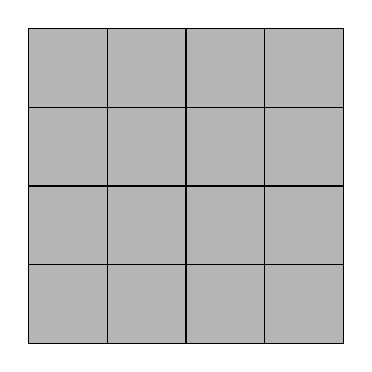
\begin{tikzpicture}
  \filldraw[fill=sqGray,draw=black,line width=0.5pt] (0.0000,0.0000) rectangle (1.0000,1.0000);
  \filldraw[fill=sqGray,draw=black,line width=0.5pt] (1.0000,0.0000) rectangle (2.0000,1.0000);
  \filldraw[fill=sqGray,draw=black,line width=0.5pt] (2.0000,0.0000) rectangle (3.0000,1.0000);
  \filldraw[fill=sqGray,draw=black,line width=0.5pt] (3.0000,0.0000) rectangle (4.0000,1.0000);
  \filldraw[fill=sqGray,draw=black,line width=0.5pt] (0.0000,1.0000) rectangle (1.0000,2.0000);
  \filldraw[fill=sqGray,draw=black,line width=0.5pt] (1.0000,1.0000) rectangle (2.0000,2.0000);
  \filldraw[fill=sqGray,draw=black,line width=0.5pt] (2.0000,1.0000) rectangle (3.0000,2.0000);
  \filldraw[fill=sqGray,draw=black,line width=0.5pt] (3.0000,1.0000) rectangle (4.0000,2.0000);
  \filldraw[fill=sqGray,draw=black,line width=0.5pt] (0.0000,2.0000) rectangle (1.0000,3.0000);
  \filldraw[fill=sqGray,draw=black,line width=0.5pt] (1.0000,2.0000) rectangle (2.0000,3.0000);
  \filldraw[fill=sqGray,draw=black,line width=0.5pt] (2.0000,2.0000) rectangle (3.0000,3.0000);
  \filldraw[fill=sqGray,draw=black,line width=0.5pt] (3.0000,2.0000) rectangle (4.0000,3.0000);
  \filldraw[fill=sqGray,draw=black,line width=0.5pt] (0.0000,3.0000) rectangle (1.0000,4.0000);
  \filldraw[fill=sqGray,draw=black,line width=0.5pt] (1.0000,3.0000) rectangle (2.0000,4.0000);
  \filldraw[fill=sqGray,draw=black,line width=0.5pt] (2.0000,3.0000) rectangle (3.0000,4.0000);
  \filldraw[fill=sqGray,draw=black,line width=0.5pt] (3.0000,3.0000) rectangle (4.0000,4.0000);
  \draw[draw=black,line width=0.6pt] (0,0) rectangle (4.0000,4.0000);
\end{tikzpicture}
\end{document}
